
%header and footer for separate chapter files

\ifx\whole\undefined
\documentclass[12pt, leqno]{book}
\usepackage{graphicx}
\input style-for-curves.sty
\usepackage{hyperref}
\usepackage{showkeys} %This shows the labels.
%\usepackage{SLAG,msribib,local}
%\usepackage{amsmath,amscd,amsthm,amssymb,amsxtra,latexsym,epsfig,epic,graphics}
%\usepackage[matrix,arrow,curve]{xy}
%\usepackage{graphicx}
%\usepackage{diagrams}
%
%%\usepackage{amsrefs}
%%%%%%%%%%%%%%%%%%%%%%%%%%%%%%%%%%%%%%%%%%
%%\textwidth16cm
%%\textheight20cm
%%\topmargin-2cm
%\oddsidemargin.8cm
%\evensidemargin1cm
%
%%%%%%Definitions
%\input preamble.tex
%\input style-for-curves.sty
%\def\TU{{\bf U}}
%\def\AA{{\mathbb A}}
%\def\BB{{\mathbb B}}
%\def\CC{{\mathbb C}}
%\def\QQ{{\mathbb Q}}
%\def\RR{{\mathbb R}}
%\def\facet{{\bf facet}}
%\def\image{{\rm image}}
%\def\cE{{\cal E}}
%\def\cF{{\cal F}}
%\def\cG{{\cal G}}
%\def\cH{{\cal H}}
%\def\cHom{{{\cal H}om}}
%\def\h{{\rm h}}
% \def\bs{{Boij-S\"oderberg{} }}
%
%\makeatletter
%\def\Ddots{\mathinner{\mkern1mu\raise\p@
%\vbox{\kern7\p@\hbox{.}}\mkern2mu
%\raise4\p@\hbox{.}\mkern2mu\raise7\p@\hbox{.}\mkern1mu}}
%\makeatother

%%
%\pagestyle{myheadings}

%\input style-for-curves.tex
%\documentclass{cambridge7A}
%\usepackage{hatcher_revised} 
%\usepackage{3264}
   
\errorcontextlines=1000
%\usepackage{makeidx}
\let\see\relax
\usepackage{makeidx}
\makeindex
% \index{word} in the doc; \index{variety!algebraic} gives variety, algebraic
% PUT a % after each \index{***}

\overfullrule=5pt
\catcode`\@\active
\def@{\mskip1.5mu} %produce a small space in math with an @

\title{Personalities of Curves}
\author{\copyright David Eisenbud and Joe Harris}
%%\includeonly{%
%0-intro,01-ChowRingDogma,02-FirstExamples,03-Grassmannians,04-GeneralGrassmannians
%,05-VectorBundlesAndChernClasses,06-LinesOnHypersurfaces,07-SingularElementsOfLinearSeries,
%08-ParameterSpaces,
%bib
%}

\date{\today}
%%\date{}
%\title{Curves}
%%{\normalsize ***Preliminary Version***}} 
%\author{David Eisenbud and Joe Harris }
%
%\begin{document}

\begin{document}
\maketitle

\pagenumbering{roman}
\setcounter{page}{5}
%\begin{5}
%\end{5}
\pagenumbering{arabic}
\tableofcontents
\fi



\chapter{Monodromy of hyperplane sections}\label{uniform position}

\section{Uniform position and monodromy} \label{uniformSection}
We now return to the situation where the ground field $k$ is algebraically
closed of characteristic 0.

The central result of this chapter is the  
\emph{uniform position lemma}, 
\index{uniform position lemma}%
which deals with the monodromy group 
of the points of a general
hyperplane section of a curve $C \subset \PP^r` `$. To define the
monodromy group  and prove the  uniform position lemma, we will use the
classical topology. An equivalent algebraic definition is described in
Cheerful Fact~\ref{Galois equals monodromy} below, but the strong form
of uniform position can fail in positive characteristic,
as shown by the examples in Exercise~\ref{strange curves}.

We may describe the 
\blue{monodromy group}
\index{monodromy group|(}%
informally as follows: Suppose that
$C \subset \PP^r$ is an irreducible curve of degree $d$ over $\CC$,
and $H_0 \subset \PP^r$ a hyperplane transverse to $C$; say $C \cap
H_0 = \{p_1,\dots,p_d\}$. As we vary $H_0$ continuously along a real
arc $\{H_t\}$, staying within the open subset $U \subset (\PP^r)^*$
of hyperplanes transverse to $C$, we can ``follow'' each of the points
$p_i(t)$ of intersection of $C$ with the hyperplane $H_t$.

Now imagine that the hyperplanes $H_t$ come back to the original $H_0$
at time $t=1$; that is, we have a continuous family $\{H_t\}_{0 \leq
t \leq 1} \subset U$ with $H_1 = H_0$. Each of the points $p_i$ then
traces out a continuous real arc
$\{p_i(t) \in C \cap H_t\}_{0 \leq t \leq 1}$. Since $H_1 = H_0$, the
end point $p_i(1)$ is one of the original points $p_j \in C \cap H_0$. In
this way, we get a permutation of the set $C \cap H_0$; the group of all
permutations arrived at in this way is called the \emph{monodromy group}
\index{monodromy group|defi}%
of the points $C \cap H_0$.

We will now give a precise definition of the monodromy group in a more
general setting, and prove that the monodromy group of the points of a
general hyperplane section of an irreducible curve
 is the full symmetric group; this is the uniform position lemma. The
 rest of the chapter 
\redden{has}
a series of applications.

\subsection*{The monodromy group of a generically finite morphism}

Let $f : Y \to X$ be a 
\blue{dominant map between varieties of the same dimension}
\index{dominant map!between varieties of same dimension}
over $\CC$, and suppose that $X$ is irreducible. There is then
a Zariski open subset $U \subset X$ such that $U$ and
its preimage $V = f^{-1}(U)$ are smooth, and the restriction of $f$
to $V$ is a covering space in the classical topology. Let $d$ be the
\index{sheets, number of}%
number of sheets. This is the degree of the extension $K(Y)/K(X)$.

\blue{Homotopy theory}
\index{homotopy theory}%
associates a monodromy group to any finite
topological covering map $f : V \to U$, defined as follows: Choose a
basepoint $p_0 \in U$, and suppose $\Gamma \colonequals  f^{-1}(p_0)  =
\{q_1,\dots,q_d\}$. If $\gamma$ is any loop in $U$ with basepoint $p_0$,
for any $i = 1, \dots, d$ there is a unique lifting of $\gamma$ to an
arc $\tilde \gamma_i$ in $V$ with initial point $\tilde \gamma_i(0)
= q_i$ and end point $\tilde \gamma_i(1) = q_j$ for some $j \in
\{1,2,\dots,d\}$. Since we could traverse the loop in the opposite
direction, the index $j$ determines $i$, and the map $i\mapsto j$ is a
permutation of $\{1,2,\dots,d\}$.
Since the set $\Gamma$ is discreet, the permutation depends only on the
class of $\gamma$ in $\pi_1(U,p_0)$, so we have defined a homomorphism
to the 
\blue{symmetric group:}
\index{symmetric group}%
$$
\pi_1(U,p_0)  \to \mathrm{ Perm}\,\Gamma \cong S_d.
$$
The image of this map,
\marginpar{since the notation is not used here}
\redden{usually denoted by $M$,} 
is called the \emph{monodromy group} of the
\index{permutation group|see symmetric group, $S_n$}%
map $f$. It depends on the labeling of the points of $\Gamma$, but a
change in labeling
only changes the group by conjugation with the corresponding permutation,
so the monodromy group is well defined up to
conjugation in $S_{d}$.
\vspace*{3pt}

\begin{fact}\label{Galois equals monodromy}
In our setting  the monodromy group is independent of the choice of open
set $U$: if $U' \subset U$ is a Zariski open subset, the complement of
$U\setminus U'$ has
real codimension $\geq 2$ so the map $\pi_1(U', p_0) \to \pi_1(U,p_0)$
is surjective. Thus the image of $\pi_1(U', p_0)$ in $S_d$ is the same.

The theory of finite coverings of algebraic varieties is not only
analogous to 
\index{Galois theory,}
it \emph{\bfseries{is}} Galois theory: In the situation
described above, if $Y$ is irreducible, then the pullback map $f^*$
expresses the function field $K(Y)$ as a finite algebraic extension of
$K(X)$. The monodromy group of $f$  is the Galois group of the Galois
\index{Galois normalization}%
normalization of $K(Y)$ over $K(X)$ (see \cite{Harris1979}). Indeed,
in early treatments of Galois theory, such as 
\redden{Camille Jordan's}
\marginpar{dropped ``originally published in 1870'' (and included info about reprint in bib entry)}
famous \emph{Trait\'e
\index{Jordan, Camille}%
des substitutions} \citeyear{MR1188877}, 
function fields played as large a role as number fields.
\index{function field}%
\index{number field}%
\end{fact}

Since we assumed that $X$ is irreducible, the space $U$ is (path)
connected, and it follows that the monodromy group is transitive if and
\index{monodromy group!transitive}%
only~if the space $V$ is (path) connected. But $V$ is a smooth
variety, so this is the case if and only~if $V$ is irreducible. For
example, the monodromy in the family
of 
\blue{smooth quadric surfaces in $\PP^3$}
interchanges the two 
\blue{rulings:}
\index{ruling!interchange of --s}%
\index{quadric surfaces!in $\PP^3$}%

\begin{example}\label{monodromy of rulings}
Consider the family
$$
X \colonequals  \big\{@(p,Q) \mid p\in Q\hbox{ a point on a smooth quadric
surface in $\PP^3$}@\big\}
$$
of pointed smooth quadric surfaces in $\PP^3$ and the double covering by
$$
V\colonequals  \big\{@((p,Q), L)\mid (p,Q)\in X,\ L \hbox{ a line with $p
\in L\subset Q$}@\big\}.
$$
The variety $V$ is irreducible: if we project $V$ to the (irreducible)
variety of lines in $\PP^3` `$,
the fiber consists of a point on the line and quadric containing the
line\emdash that is, the product
of $\PP^1$ and the (dual of the) projective space
on the space of quadratic forms in the ideal of the line. Thus the
monodromy of the family
is transitive, and exchanges the two lines through the point.
\end{example}

\subsection*{Uniform position}


We will next compute the monodromy group of the  universal hyperplane
section of a curve, constructed as follows:
Let $C \subset \PP^r$ be an irreducible, nondegenerate curve of degree
$d$, and let $X = (\PP^r)^*$ be the space of hyperplanes in $\PP^r``$. 
We define the \emph{universal hyperplane section} of $C$ to be the
\index{universal hyperplane section|defi}%
projection  $f: Y\to (\PP^r)^*$ of the incidence variety
$$
Y = \{ (H, p) \in (\PP^r)^* \times C \mid p \in H \}.
$$
The fibers of $f$ are the hyperplane
sections of $C$, so $f$ is a finite surjective map. If we let $U\subset
(\PP^r)^*$ be the open subset of hyperplanes
meeting $C$ transversely, then the restriction of $f$ to the preimage $V$
of $U$ is a covering space
whose fibers each consist of $d$ distinct points. The preimage in $Y$
of a point $p\in C$ is the set of hyperplanes containing
$p$, a copy of $\PP^{r-1}$, and thus $Y$ is irreducible. Thus the
monodromy group of $f$ is transitive. But much more is true:

\begin{theorem}[uniform position lemma]
\label{uniform position lemma}
The 
\marginpar{theorem $\to$ lemma (since that's what you've called it elsewhere)}
monodromy group of the universal hyperplane section of an irreducible
curve $C \subset \PP^r$ is the full symmetric group~$S_d$.
\index{symmetric group}%
\end{theorem}

We postpone the proof to develop some necessary tools.

Theorem~\ref{uniform position lemma} fails over fields of finite
characteristic, though there is no known counterexample for smooth
curves; see Exercise~\ref{strange curves} for singular examples, and
\cite{Rathmann} and \cite{Kadets} for what is known.

Theorem~\ref{uniform position lemma} implies that two subsets of the
same cardinality in the general hyperplane section of $C$
are indistinguishable from the point of view of any discrete invariant
that is semicontinuous in the Zariski topology. To make this precise,
we introduce a definition:

\begin{definition}
Let $\phi : Y \to X$ be a finite morphism. By the 
\emph{restricted fiber power} 
\index{restricted fiber power|defi}%
$\tilde Y^n`/X$ we will mean the complement of all diagonals in
the ordinary fiber power; that is,
$$
\tilde Y^n`/X \colonequals  \bigl\{@ (x, y_1,\dots, y_n) \in X \times Y^n \mid
\phi(y_i) = x \text{ and } y_i \neq y_j \; \forall i \neq j @\bigr\}
$$
\end{definition}

In down-to-earth terms, a point of $\tilde Y^n`/X$ is a set of $n$
distinct points in a fiber of $\phi$ together with
the choice of a total order on these points.

\begin{lemma}\label{transitivity lemma}
Let $f : Y \to X$ be a generically finite cover of degree $d$, with
monodromy group $M \subset S_d$.
$M$ is $n$-transitive if and only~if the restricted fiber power $\tilde
Y^n`/X$ is irreducible.
\end{lemma}

\begin{proof}
If we restrict ourselves to open subsets $U \subset X$ and $V = f^{-1}(U)
\subset Y$ such that $U$ and $V$ are smooth and the restriction $f|_V :
V \to U$ is a covering in the classical topology, then the restricted
fiber powers are unions of connected components of the usual fiber
powers $Y^n`/X$. The condition that the monodromy is $n$-transitive is
equivalent to the condition that the restricted fiber power $\tilde Y^n`/X$
is connected; since the fiber powers are all smooth, this is equivalent
to $\tilde Y^n`/X$ being irreducible.
\end{proof}



\section{Flexes and bitangents are isolated}\label{isolated flexes
and bitangents}

There are  further general position results that we need for the proof
of the uniform position lemma.  We have separated
them from the results on linear general position because these require
characteristic 0; they are really local analytic
statements.

\subsection*{Not every tangent line is tangent at a flex}

%\label{isolated tangents and bitangents}

Recall that a smooth point $p$ on a curve $C \subset \PP^r$ is called
a \emph{flex point} if the tangent line to $C$ at  $p$ has contact of
\index{flex point}%
order 3 or more with $C$ at $p$.

\begin{lemma}\label{finite inflections}
If $r>1$ and $C \subset \PP^r$ is a smooth, irreducible and nondegenerate
curve, then not every point of $C$ is a flex point.
\unif
\end{lemma}

The proof applies to any linear series on a curve.
\unif

\begin{proof}
We begin by lifting the inclusion $C \hookrightarrow \PP^r$ to an arc
$v (t)$ in $\CC^{r+1}$, so that the tangent line at the point $t=0$
in projective space
is represented by the span of $v(0)$ and $v'(0) \in \CC^{r+1}$. To say
that $v(t)$ is a flex point is to say that the  vectors $v(t), v'(t)$
and $v''(t)$ are linearly dependent. If this holds for all $t$ then
$$
v(t) \wedge  v'(t) \wedge v''(t) \; \equiv \; 0.
$$

When we take the derivative of the wedge product $v(t) \wedge v'(t)
\wedge v''(t)$ by applying the product rule we see that the first two
terms are zero because they contain a repeated factor; it follows that
$$
v(t) \wedge  v'(t) \wedge v'''(t) \equiv 0,
$$
so that $v'''(t)$ lies in the span of $v(t)$ and $v'(t)$ as well. Indeed,
as we continue to take derivatives, we see in each case that all but one
term is zero, and we deduce that $v^{(l)}(p)$ lies in the span of $v(t)$
and $v'(t)$ for all $l$. This being characteristic 0, it follows that $C$
lies in a line, contrary to our hypothesis.
\end{proof}


\subsection*{Not every tangent is bitangent}

 This statement seems even more obvious than Lemma~\ref{finite
 inflections} above, but, like that lemma, it is false in
\marginpar{normalized punctuation}
 characteristic $p$\emdash see Exercise~\ref{kaji}.


 \begin{lemma}\label{tangent not bitangent}
 Let $C \subset \PP^r$ be a smooth, irreducible, nondegenerate curve,
 with $r > 1$. If $p \in C$ is a general point, then the tangent line
 $\TT_p(C) \subset \PP^r$ is not tangent to $C$ at any other point.
\unif
 \end{lemma}

 \begin{proof} Again the result is local, this time with a pair of germs
 $D\ruto {\ v} ` `\PP^r$ and $D\ruto {\,w} ` `\PP^r` `$. If every
 tangent line to the two curves is a bitangent, we will show that they
 are both contained in a line.

  Let $C_1, C_2$ be the images of $v,w$ respectively, and let $\tilde v,
  \tilde w$ be lifts to $\CC^{r+1}$.
 Let
 $$
 \Sigma \colonequals  \bigl\{@ (p,q) \in D \times D \mid \text{ and
 }\TT_{v(p)}(C_1) = \TT_{w(q)}(C_2)@ \bigr\}
\marginparhere{\redden{Is there something missing before ``and''?}}
 $$
 be the variety parametrizing bitangents to the two germs.



 The statement that the tangent lines to $C$ at the points $v(t)$
 and $w(t)$ are equal then says that the vectors $\tilde v(t), \tilde
 v'(t),\tilde w(t)$ and $\tilde w'(t)$ all lie in a 2-dimen\-sional subspace
 $\Lambda \subset \CC^{r+1}$; in particular,
 $$
 \tilde v(t) \wedge \tilde v'(t) \wedge \tilde w(t) \equiv 0 \quad
 \text{and likewise} \quad \tilde v(t) \wedge \tilde w(t) \wedge \tilde
 w'(t) \equiv 0
.
 $$

We proceed now exactly as in the proof of Lemma~\ref{finite inflections}:
taking derivatives, we see that all derivatives of $\tilde v(t)$
and $\tilde w$ at $t=0$ lie in $\Lambda$
and hence $C_1$ and $C_2$ are both contained in the line in $\PP^r$
corresponding to $\Lambda$.
 \end{proof}

In characteristic zero, \cite[Theorem 3.1]{kaji-tangentialDegeneracy}
shows that a general tangent line to a smooth projective curve $C$ can
intersect $C$ in a point other than $p$, except of course in case $r=2$,
although this is possible in characteristic $p>0$.

\section{Proof of the uniform position 
\redden{lemma}
}

Let $C \subset \PP^r$ be an irreducible, nondegenerate curve of degree $d$
and 
\marginpar{displayed for better layout, and added ``let\dots be'' for fluency}
\redden{let}
$$f : Y \subset (\PP^r)^* \times C \to  X = (\PP^r)^*$$ 
\redden{be}
its universal
hyperplane section; let $U \subset (\PP^r)^*$ be the open subset of
hyperplanes transverse to $C$ and $V = f^{-1}(U)$; let $M \subset S_d$
be the monodromy group of $V$ over $U$.
To show that  $M$ is the full symmetric group, it suffices to show that
$M$ contains all transpositions, and for this it is enough to show that
\index{doubly transitive}%
$M$ is doubly transitive and contains one transposition.

To prove that $M$ is doubly transitive, we can give a concrete description
\vadjust{\allowbreak}%
of the restricted fiber power $\tilde V^2`/U$: let
\index{restricted fiber power}%
$$
\Sigma \colonequals  \bigl\{@ (H, p, q) \in (\PP^r)^* \times C \times C
\mid p, q \in H \text{ and } p \neq q @\bigr\}.
$$
Projection on the second and third factors expresses $\Sigma$ as a
$\PP^{r-2}$-bundle over the complement $C \times C \setminus \Delta$
of the diagonal in $C \times C$. Thus $\Sigma$ is irreducible, and it
follows that the restricted fiber square $\tilde V^2`/U$, which is a
Zariski open subset of $\Sigma$, is as well. Note that this part of the
argument does not rely on any assumption about the characteristic.

Next we give a criterion for a monodromy group to contain a transposition:

\begin{lemma}\label{transposition lemma}
Let $f : Y \to X$ be a generically finite cover of degree $d$ over an
\index{transposition}%
irreducible variety $X$, with  monodromy group $M \subset S_d$.
If,  for some smooth point $p \in X$ the fiber $f^{-1}(p)\subset V$
consists of $d-2$ reduced points $p_1,\dots, p_{d-2}$ and one point $q$
of multiplicity \2, where $q$ is also a smooth point of $Y$, then $M$
contains a transposition.
\end{lemma}

\begin{figure}
\centerline {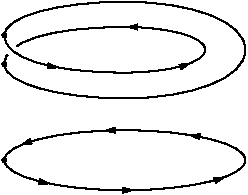
\includegraphics[height=1.4in]{main/Fig10-1}}
\vskip-5pt
\caption{Monodromy action around the ramification point of a double cover.}
\label{$d=2$ monodromy}
\end{figure}

See Figure~\ref{$d=2$ monodromy} for the case $d=2$.

\begin{proof} 
The hypothesis implies that $Y$ is smooth
\marginpar{dropped ``Note that''}
locally near the fiber over $p$. Let $U \subset X$ be a Zariski open
subset of the smooth locus in $X$, as in the definition of the monodromy
group, so that  $V \colonequals  f^{-1}(U)$ is also smooth and the
restriction $f|_V : V \to U$ expresses $V$ as a finite $d$-sheeted
covering space of $U$, with $U,V$ smooth and $p\in X$.

Let $B_i\subset Y$ be disjoint small connected closed neighborhoods of
the points
in $f^{-1}(p)$. Because $f|_V$  is finite, the image $A \colonequals
\bigcap f(B_i)$  is a locally
closed subset of the same dimension as $X$ and thus $A$
 contains a neighborhood
of $p$ in the classical topology.

Let $p' \in A \cap U$. Two of the $d$ points of $f^{-1}(p')$  lie in the
component  of $B$ containing $q$; call these $q'$ and $q''$. Since $B
\cap V$ is the complement of a proper subvariety in $B$ it is connected,
and we can draw a real arc $\gamma : [0,1] \to B \cap V$ joining $q'$
to $q''$; by construction, the permutation of $f^{-1}(p')$ associated
to the loop $f \circ \gamma$ will exchange $q'$ and $q''$ and 
\redden{fix} 
\marginpar{or else ``exchanges''}
each
of the remaining $d-2$ points of $f^{-1}(p')$.
\end{proof}

\begin{proof}[Completion \kern1.5pt of \kern1.5pt the \kern1.5pt proof \kern1.5pt of \kern1.5pt the \kern1.5pt uniform \kern1.5pt position \kern1.5pt lemma]
\redden{What is left to show is}
\marginpar{to allow line break}%
that a reduced irreducible curve $C$ of degree $d$
 (in characteristic 0)
 has a hyperplane section consisting of $d-2$ smooth points and one
 double point; that is, a hyperplane simply tangent to the curve at one
 point and transverse everywhere else. By the results of
 Section~\ref{isolated flexes and bitangents} there is a tangent line $L$
 to $C$ at a smooth point that is not flex tangent, and is not tangent
 to $C$ at any other point. A general hyperplane $H$ containing $L$
 meets $C$ doubly in the point of
 tangency. At any other point $p$ of $L\cap C$, if any, the intersection
 $C\cap H$ is transverse
 unless $H$ contains the tangent line at $p$. Containing such a line is
 a  proper codimension 1 condition on
 the hyperplanes containing $L$, and since there can only be finitely
 many such points, a
 general  $H$ will be transverse at all such $p$. On the other hand,
 at points not on $L$
 the intersection $H\cap C$ is transverse by Bertini's theorem. This
 completes the proof.
\end{proof}

\subsection*{Uniform position for higher-dimensional varieties}

\redden{There is}
a generalization of Theorem~\ref{uniform position lemma}
for irreducible varieties $X \subset \PP^r$ of any dimension $k$. To set
this up, let $\GG(r-k,r)$ be the 
\blue{Grassmannian}
\index{Grassmannian}%
parametrizing $(r-k)$-planes
$\Lambda \subset \PP^r` `$. We introduce the \emph{universal $(r-k)$-plane
section of} $X$:
$$
Y = \{ (\Lambda, p) \in \GG(r-k,r) \times X \mid p \in \Lambda \}.
$$
\redden{Via}
\marginpar{to allow line break}
projection on the first factor, $Y$ 
\redden{can be expressed} as a generically finite
cover of $\GG(r{@-@}k,r)$, and we can ask for its monodromy. The answer is
the same as for curves:


\begin{theorem}\label{higher dim uniform position lemma}
The monodromy group of the universal $(r-k)$-plane section of an
\index{monodromy group}%
\index{universal plane section}%
of the universal $(r-k)$-plane section of an
irreducible $k$-dimensional variety $X \subset \PP^r$ is the full
\index{symmetric group}%
\blue{symmetric group}
$S_d$.
\end{theorem}

\begin{proof}
This follows from Theorem~\ref{uniform position lemma}.
\marginpar{removed ``In fact'' etc. to avoid breaking inside $(r-k+1)$}
\redden{To see this},
fix a general $(r-k+1)$-plane $\Gamma \subset \PP^r$; since a
general hyperplane section of an irreducible variety $X \subset \PP^r$
of dimension $k \geq 2$ is again irreducible, we see that $C \colonequals
\Gamma \cap X$ is an irreducible curve. The restriction of the universal
$(r-k)$-plane section of $X$ to the sub-Grassmannian $\GG(r{@-@}k, \Gamma)
\cong (\PP^r)^*$ of $(r{@-@}k)$-planes contained in $\Gamma$ is just the
universal hyperplane section of the curve $C$, which we know has monodromy
$S_d$; since the monodromy group of a cover can only get smaller under
restriction to a subvariety of the target, the result follows.
\end{proof}

We will see an application of this result in 
\marginpar{\leftskip-65pt dropped ``below'' (``will'' is enough :-). \redden{the label here was that of a subsection, not a proposition; but by good fortune (?) the two things had the same number 11.4.4, so I think it's all good now.}}
Proposition~\ref{plane curve nodes}.

\section{Applications of uniform position}
\subsection*{Irreducibility of fiber powers}

If we apply the uniform position lemma to the universal hyperplane
section of a curve $C \subset \PP^r$ we get an irreducibility result:

\begin{corollary}\label{hyperplane section monodromy} If $C\subset \PP^r$
is a smooth curve of degree $d$, then
for $k\leq d$, the restricted fibered powers $\tilde Y^k`/X$  of the
universal hyperplane section
of $C$ are irreducible.
\end{corollary}

\subsection*{Numerical uniform position}

The property of uniform position, as exposed above, is really a property
of a family --- the irreducibility of the restricted
fiber powers --- and not of a given set of points. There is a useful
weaker property that
can be applied to a given set of points:

\begin{definition}
 A set of points $\Gamma\subset \PP^n$ is in \emph{numerical uniform
 position} if
 any two subsets of $\Gamma$ with the same cardinality impose the same
 number of conditions on forms of any degree; that is, any two subsets
 of the same cardinality have the same Hilbert function.
%
\begin{figure}
\leavevmode
\vbox{\offinterlineskip
\hbox{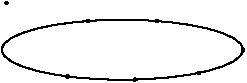
\includegraphics[scale=1.3,viewport=-10 37 118 39,clip]{main/Fig10-2}}%
\hbox{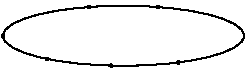
\includegraphics[scale=1.3,viewport=0 0 118 33,clip]{main/Fig10-2a}}}
\caption{
\redden{Seven}
points in the plane,
\redden{of which six}
on a conic, in linearly general 
\redden{position}
but not 
\redden{in numerical}
uniform position.}
\label{numerical uniform is stronger}
\end{figure}
%
(This is strictly stronger than linearly general position, as illustrated
\marginpar{moved this sentence here, parenthetically}
in Figure~\ref{numerical uniform is stronger}.)
\end{definition}

\begin{corollary}[numerical uniform position lemma]\label{numerical
uniform position lemma}
The general hyperplane section of an irreducible curve
\index{numerical uniform position lemma}
$C\subset \PP^r$ is in numerical uniform position.
\unif
\end{corollary}

\begin{proof} Let $U = (\PP^r)^* \setminus C^*$ be the open subset
of hyperplanes transverse to $C$, and let $Y\to U$ be the universal
hyperplane section.
Corollary~\ref{hyperplane section monodromy} says that the restricted
fiber powers $\tilde V^n`/U$ are irreducible.

Now, for each $m$ the number of conditions that $\Gamma$ imposes on
forms of degree $m$ is lower semicontinuous, so it achieves its maximum
on a Zariski open subset of $\tilde V^n`/U$. Since $\tilde V^n`/U$ is
irreducible, the complement $Z$ of this open set has dimension strictly
less than $\dim \tilde V^n`/U = \dim U$. Thus a general hyperplane $H
\in (\PP^r)^*$  lies outside the image of $Z$, meaning that the number
of conditions imposed by all the $k$-element subsets $\Gamma \subset C
\cap H$ have this maximal value.
\end{proof}

This result may be seen as an important strengthening of
Theorem~\ref{basic linear independence}, since if $C$ is a reduced,
irreducible nondegenerate curve in $\PP^n$ then a general subset
of $n$ points of $C$ is linearly independent and spans a hyperplane;
Corollary~\ref{numerical uniform position lemma} says that this 
\redden{holds}
for every subset of $n$ points of every general hyperplane section,
which reproves Theorem~\ref{basic linear independence}, though only in
characteristic~0.

\subsection*{Sums of linear series}

Another consequence of the uniform position lemma is a result about sums
\index{linear series!sums of}
of linear series.
Recall that if $D$ is a divisor on a curve $C$ we write $r(D) = \dim |D|
= h^0(\cO_C(D))-1$.

\begin{corollary}\label{Clifford equality plus}
If $D,E$ are effective divisors on a curve $C$ then
$$
r(D+E) \geq r(D)+r(E).
$$
If the genus of $C$ is $>0$ and $|D+E|$ is 
\blue{birationally very ample,}
\index{birationally very ample}%
\index{very ample!birationally}%
then the inequality is strict.
\end{corollary}

On $\PP^1` `$, by contrast, any effective divisor $D$ has $r(D) = \deg
D$, so the inequality above is
always an equality for $C = \PP^1` `$.

\begin{proof}
 The inequality follows in general because the sums of divisors in $|D|$
 and divisors in $|E|$ already move in
 a family of dimension $r(D)+r(E)$; the key point is the strict inequality
 in case $D+E$ is birationally very ample.

If $D+E$ is birationally very ample and $r(D+E) = r(D)+r(E)$ then
restricting to an open set
we may identify $C$ with its image under the complete linear series
$|D+E|$, and we see that a general hyperplane section $H\cap C$ contains
a divisor equivalent to $D$.

Let $Y$ be the $\deg D +\deg E$ restricted fiber power of the universal
hyperplane.
A point $y\in Y$ is a hyperplane section plus an ordering of its points.
Let $\phi: Y \to \Pic_d(C)$ be the 
\blue{Abel--Jacobi map}
\index{Abel--Jacobi map}%
 taking $y$
 to the class of the divisor that is the sum of first $d$ points in this
 order. The preimage  $Y'$ of the point of $\Pic_d(C)$ corresponding to
 the class of $D$ is a closed subset, and
since every divisor in the class of a hyperplane section contains
a divisor
linearly equivalent to  $D$, the subvariety $Y'$ dominates $(\PP^{n})^*$,
and thus
has the same dimension as~$Y$. Consequently $Y'=Y$, and the sum of the
first $d$ points
in any ordering of the general hyperplane section\emdash that is, the
sum of any $d$
of the points\emdash is equivalent to $D$.

Thus if $p\in D$ and $q\notin D$, then $D-p+q \equiv D$, whence $q\equiv
p$. Thus
$r(p)\geq 1$, so $C\cong \PP^1$.
\end{proof}

\subsection*{Nodes of plane curves}

\def\VD#1{V_{\mskip-5mu d,#1}} % compensate for huge gap in V_{d}

In Section~\ref{severi variety}, we introduced the \emph{Severi variety}
\index{Severi variety}%
$\VD{g}$; this is the locally closed subset of the projective space
$\PP^N$ of all plane curves of degree $d$ parametrizing irreducible
\marginpar{dropped $\delta:=$ to allow line break; it was anyway redefined again each time, except right after the next display, and in that case I expanded it (red expression below).}
plane curves of degree $d$ having 
$\tbinom{d-1}{2} - \nobreak g$ 
nodes and no other singularities. We proved there that $\VD{g}$ was
smooth, and by Cheerful Fact~\ref{severi irreducible} it is irreducible
for all $d$ and $g$.

To compute the monodromy we introduce the incidence correspondence
$$
\Phi \colonequals \big\{@(C, p) \in \VD{g} \times \PP^2 \mid p \in C_{\sing}
@\big\}.
$$
This is a
covering space of $\VD{g}$
\redden{with $\tbinom{d-1}{2} - \nobreak g$ sheets,} 
and we compute its
monodromy. We start with the extremal case $g = 0$:
\marginpar{\leftskip-130pt \hangindent 130pt \hangafter 2 dropped extra ``is'' after ``monodromy'' (or did you mean to write ``what its monodromy is''?); replaced hanging ``where we can prove'' by colon\parfillskip0pt\endgraf}

\begin{proposition}
The monodromy group of $\Phi$ over $\VD{0}$ is the full symmetric group
\label{plane curve nodes}
$S_\delta$, with $\delta = \tbinom{d-1}{2}$.
\end{proposition}

\begin{proof}
Every 
\blue{nodal curve}
\index{nodal curve}%
$C \subset \PP^2$ is the projection of a
\blue{rational normal curve}
\index{rational normal curve}%
$\tilde C \subset \PP^d$ from a $(d-3)$-plane
$\Lambda \subset \PP^d` `$. Moreover, if $\Lambda$ is general,  the nodes
of the projection correspond to the points of intersection of $\Lambda$
with the  
\blue{secant variety}
\index{secant variety}%
$X \subset \PP^d$ of the rational normal curve
$\tilde C$. Applying Theorem~\ref{higher dim uniform position lemma},
the result follows.
\end{proof}

This result has an immediate consequence, which played a major role in the
proof of Cheerful Fact~\ref{severi irreducible}: given the description in
Section~\ref{severi variety} of $\VD{g}$ in a neighborhood of a point
in $\VD{0}$, it follows that there is a unique irreducible component
of $\VD{g}$ containing $\VD{0}$ in its closure. Thus, to prove the
irreducibility of $\VD{g}$, it is sufficient to show that every component
of $\VD{g}$ contains $\VD{0}$ in its closure.

Going in the other direction, note also that if we assume Cheerful
Fact~\ref{severi irreducible}, then we can deduce the analogous result
for all $g$:


\begin{proposition}
The monodromy group of $\Phi$ over $\VD{g}$ is the full symmetric group
$S_\delta$, with $\delta = \tbinom{d-1}{2} - g$.
\end{proposition}



\section{Exercises}

As a consequence of Theorem~\ref{higher dim uniform position lemma},
we can deduce the 
\blue{Bertini irreducibility theorem:}
\index{Bertini irreducibility theorem}%

\begin{exercise}
Let $X \subset \PP^r$ be an irreducible variety of dimension $k \geq
2$. Show that a general hyperplane section of $X$ is irreducible.

Hint: Say $k=2$. If the general hyperplane section of $X$ were reducible,
there would be distinguished subsets of the intersection of $X$ with
a general $(r-2)$-plane $\Lambda$ (the intersections of $\Lambda$ with
the components of $H \cap X$, for $H$ a general hyperplane containing
$\Lambda$); but we know the monodromy on $X \cap \Lambda$ is the full
symmetric group.
\end{exercise}

\begin{exercise}
In Example~\ref{monodromy of rulings}, we gave a global argument to say
that in the family of smooth quadric surfaces in $\PP^3$ the monodromy
exchanges the two rulings of a quadric by lines. Prove this with a local
calculation, analyzing the family
$$
Q_t \colonequals  V(X^2+Y^2+Z^2 + tW^2)
$$
in a neighborhood of $t=0$.

Hint: Choose a basepoint of the pencil, say $p = [1, i, 0, 0]$. The
lines of the two rulings of $Q_t$ passing through $p$ are
$Y-iX = Z-\pm i@\sqrt{t}@W = 0$, which are exchanged under the monodromy
as $t$ goes around 0.
\end{exercise}

\begin{exercise}[tangential degeneracy {{\cite[Example 4.1]{kaji-tangentialDegeneracy}}}]
\label{kaji}
Show that the linear series 
\marginpar{dropped extra ``in''}
in Exercise~\ref{1,d-1 on quadric}
\index{tangential degeneracy}%
defines an isomorphism with a smooth curve $C$ of type $(1, d-1)$ on a
nonsingular quadric in $\PP^2_k$ no matter what field $k$ is chosen. Now
suppose that  $k$ has characteristic $p>0$ and $d-1 = p^\ell n$ with
\marginpar{changed $>\ge$ to $\ge$}
\redden{$\ell\ge 2$}
and $n$ relatively prime to $p$.
Show that the tangent lines to $C$ are the rulings of the quadric in the
family that meet $C$ with multiplicity $d-1$, and that the intersection of
each tangent line meets $C$ in $n$ distinct points, each with multiplicity
$p^\ell$. Thus Lemma~\ref{tangent not bitangent}
fails in 
\blue{positive characteristic.} 
\index{positive characteristic}% 
\end{exercise}

\begin{exercise}
Let $C \subset \PP^r$ be a union of irreducible curves $C_i$ of degrees
$d_i$. Prove that the monodromy group of the points of a general
hyperplane section of $C$ is the product $\prod S_{d_i}$.
\marginpar{moved hint within exercise, ok? (It will move to the end, but I just want to make sure it refers to this exercise only)}

Hint: We need to know that the dual hypersurfaces $C_i^* \subset
(\PP^r)^*$ are all distinct; given this, we can exhibit loops that induce
a given permutation of the points of $H \cap C_i$ while fixing the points
of $H \cap C_j$ for $j \neq i$. To see that the dual hypersurfaces $C_i^*
\subset (\PP^r)^*$ are all distinct, invoke the duality theorem $(C_i^*)^*
= C_i$ (see for example \cite{3264}).
\end{exercise}

\begin{exercise}
Let $d$ and $e$ be positive integers, $\PP^M$ the space of plane curves
of degree $d$ and $\PP^N$ the space of plane curves of degree $e$, and
$$
\Phi \colonequals  \big\{@ (D, E, p) \in \PP^M \times \PP^N \times \PP^2 \mid
p \in D \cap E@\big \}.
$$
Prove that the monodromy group of the projection $\pi : \Phi \to \PP^M
\times \PP^N$ is the symmetric group $S_{de}$ on $de$ letters
\begin{enumerate}
\item by applying Theorem~\ref{uniform position lemma}; and
\item from scratch, using the method used in the proof of
Theorem~\ref{uniform position lemma}.
\end{enumerate}

Hint: for the first part, we can fix the curve $E$ and prove the
a priori stronger statement that the monodromy on the points of
$D \cap E$ as $D$ varies is the symmetric group; this follows from
Theorem~\ref{uniform position lemma} applied to the Veronese embedding
$\nu_d(E)$. Alternatively, we can exhibit a transposition by finding a
pair $(D,E)$ such that $D \cap E$ consists of $de-2$ simple points and
one double point, and prove double transitivity with the usual incidence
correspondence argument.
\end{exercise}

\begin{exercise}
If $E \subset \PP^2$ is a smooth plane cubic curve, then a point $p \in E$
is  a 
\blue{flex}%
\index{flex}%
\marginpar{removed italics on flex}
if $\cO_E(3p) \cong \cO_E(1)$. By Corollary~\ref{torsion
points} in case $g=1$, there are nine of them. Now let $\PP^9$ be the
space of 
\blue{plane cubics, }
\index{plane cubics}%
and let
$$
\Phi \colonequals  \big\{@(E, p) \in \PP^9 \times \PP^2 \mid p \text{ is a
flex of } E@ \big \}.
$$
Show that the monodromy group of $\Phi \to \PP^9$ is a proper subgroup
of $S_9$.

Hint: the line joining any two flexes of a plane cubic $E$ contains
a third.
\end{exercise}

\begin{exercise}
Let $C$ be a smooth projective curve. Show that if $\pi : C \to \PP^1$
is a simply branched cover of degree $n$, then the monodromy of the map
$\pi$ is the full symmetric group $S_n$.

Hint: Show that a transitive subgroup of $S_n$ generated by 
\blue{transpositions}
\index{transposition}%
is all of $S_n$.
\index{monodromy group|)}%
\end{exercise}

\input footer.tex